\documentclass[a4paper,12pt]{scrreprt}
\usepackage[T1]{fontenc}
\usepackage[utf8]{inputenc}
\usepackage[english]{babel}
\usepackage[table]{xcolor}% http://ctan.org/pkg/xcolor
\usepackage{tabu}
\usepackage{graphicx}
\usepackage{lmodern}
\usepackage{longtable}
\usepackage{morefloats}
\usepackage{comment}

\begin{document}

 
%\titlehead{Kopf} %Optionale Kopfzeile
\author{Ahmed Aly \and Helmuth Brunner \and Stefan Pitirut } %3 Autoren
\title{TASK 02 Rock the net } %Titel/Thema
\subject{SEW} %Fach
%\subtitle{ } %Genaueres Thema, Optional
\date{\today} %Datum
\publishers{5AHITT} %Klasse

\maketitle
\tableofcontents


\chapter{Task}

\subsection{Basic tasks}

Implement a simple-to-use application to monitor and configure a hardware firewall appliance “Juniper NetScreen 5GT “. The firewall allows read access over the SNMP-protocol (your app should be able to test if SNMPv3 is available and if not fallback on SNMPv2c) and write access over Telnet.

Your app should accomplish following tasks:
\begin{itemize}

    \item List all configured firewall rules (policies) on the device, add the details of the mentioned services and zones as well.

    \item Allow refreshing of the list by clicking a button and by a configurable time-intervall. Your GUI should remain responsive even with short refresh-intervals!

    \item Visualize the thru-put for a highlighted firewall-rule (nice2have: multiple rows) in a line-chart (configurable refresh-interval, unit bytes/sec)

    \item Encapsulate the data retrieval for further reuse and easy expansion. An UML-model of your design will help you defend it at the review!

    \item Build a visual appealing and easy to use interface (there is more than Swing out there).
\end{itemize}
\subsection{Advanced tasks (obligatory for grades better than C)}

Additionally to the basic tasks your app should accomplish the following:
\begin{itemize}


    \item Alarm the user visually and per email if the config of the firewall-rules changes. To avoid polling use the SNMP-trap mechanism.

    \item Allow managing of firewall-rules (CRUD). To accomplish this, you will have to send configuration commands via telnet or ssh. An admin-account is available per request.

    \item Use multicast-groups to build a simple transaction system to serialize administrative tasks on the firewall (for example pass an “admin token” to recognize the collaborator who is allowed to write to the firewall). This should also work in a heterogenous environment (different implementations, different OSes), so you have to coordinate with other teams.

    \item Make sure, that your interface to the firewall allows an easy change of the firewall-model (new releases, manufacturer, ...). It is not necessary to make this configurable in the GUI but must (explicitly) be considered in your software-design!
\end{itemize}

	
\chapter{Design concept}
	SNMP Package:
	The SNMP package has an OIDDecoder, which defines the Standard OID's in static final variables. The OIDDecoder is now deprecated, because it is not dynamic. 
	The OID will be handelt with a new library Mibble, which will make it possible to load mib files and map them.
	\\\\
	The Factory pattern is used here to allow the class SNMPManager to use the right SNMP version. This pattern also allows the developer to add to SNMP version, if there are any new ones coming.
	\\
	The SNMP Manager sends a package with a specific OID and returns the receive message. This Class will be used as a Connector and a Receiver, which will be called by a command class.
	\\\\
	Command pattern:
	A command pattern is used to create specific actions, which can any connectors like SNMP, SSH or Telnet.
	\\\\
	Naturally there will be self written exceptions, which will be in the exceptions package.
	\\\\
	The Unit and GUI tests will be in a own test package.   
\chapter{User Stories}
As a user, I want to visually see the thru-put in bytes/sec as a chart on my Graphical User Interface.\\

As a user, I want to set the refresh-timer for the visualized thru-put on my Graphical User Interface.\\

As a user, I want to manually refresh the visualization for the thru-put on the Graphical User Interface.\\

As a user, I want to see the rules/zones/services of the firewall listed on the Graphical User Interface.\\

As a user, I want set the refresh-timer for the listing of the rules/zones/services of the firewall on the Graphical User Interface.\\

As a user, I want to manually refresh the listing of the rules/zones/services of the firewall on the Graphical User Interface.\\

As a user, I want to configure the application threw the Graphical User Interface.\\
\chapter{Libraries}
\begin{description}
\item The required libraries will be:
\begin{itemize}
\item SNMP4J
\item LOG4J
\item JUNIT
\item Mockito
\item Java Secure Channel (JSCH) |SSH|
\item JavaFX
\item Mibble
\item JavaMail
\end{itemize}
\end{description}


\chapter{Diagrams}

\subsection{Policy Design}
The policy date will be shown in a table, which consists of 9 Elements. 
\begin{description}
\item The table header would look like this:\\
{policyId} | {policyName} | {policyServiceName} | {policySrcZone} | {policyDestZone} | {policySrcAddr} | {policyDestAddr} | {policyAction} | {policyStatus}
\item OIDs:\\
\begin{tabular}{l l l} 
policyId & .1.3.6.1.4.1.3224.10.1.1.1 & branch\\
policyName & .1.3.6.1.4.1.3224.10.1.1.24 & branch\\
policyServiceName & .1.3.6.1.4.1.3224.10.1.1.25 & branch\\
policySrcZone & .1.3.6.1.4.1.3224.10.1.1.3 & branch\\
policyDestZon & .1.3.6.1.4.1.3224.10.1.1.4 & branch\\
policySrcAddr & .1.3.6.1.4.1.3224.10.1.1.5 & branch\\
policyDestAddr & .1.3.6.1.4.1.3224.10.1.1.6 & branch\\
policyAction & .1.3.6.1.4.1.3224.10.1.1.8 & branch\\
policyStatus & .1.3.6.1.4.1.3224.10.1.1.23 & branch\\
\end{tabular}

\end{description}
The next step is to draw a chart with the thru-put of the firewall-rule in a line-chart, which is possible with the value policyBps. 

\begin{description}
\item OID:\\
\begin{tabular}{l l l} 
policyBps & .1.3.6.1.4.1.3224.10.2.1.6 & branch\\
\end{tabular}
\end{description}

\subsection{UML Class Diagram}

\begin{figure}[h!]
\centering
\caption{UMLClass Diagram}
\label{fig:RTNUmlImage}
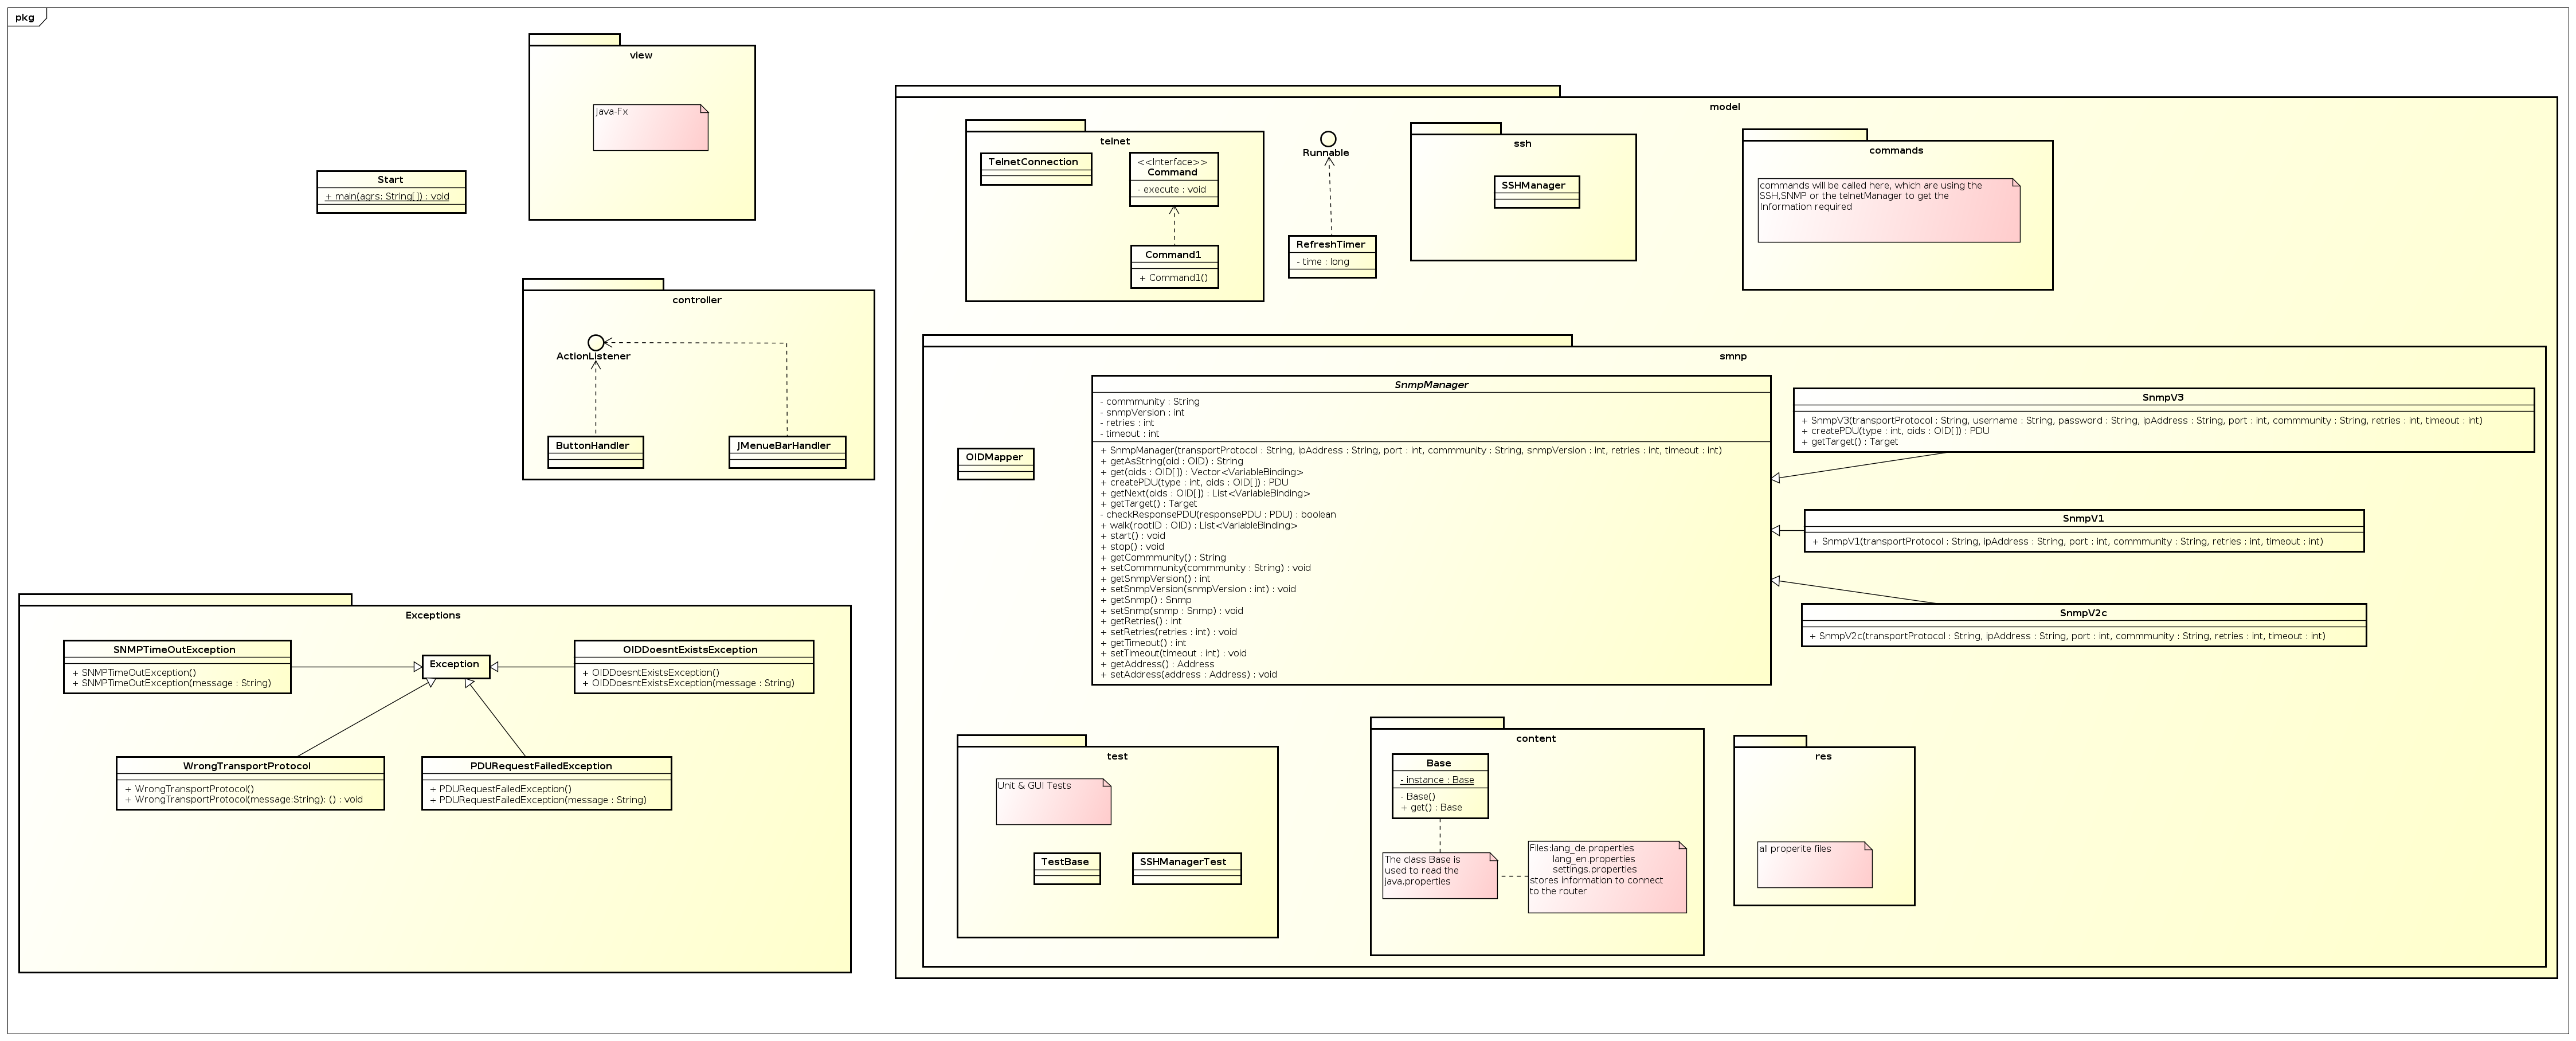
\includegraphics[angle=90,width=1.0\textwidth]{RTNUmlImage}
\end{figure}

\chapter{Time Estimation}
	%\tabulinesep = 5pt
	\begin{longtabu}  {|[2pt]X[6,c] |[1pt] X[4,c] |[1pt]X[4,c]|[1pt]X[4,c]|[1pt]X[4,c]|[1pt]X[4.5,c]|}
		\tabucline[2pt]{-}
		Packages & Time needed & Time Estimated & Description & Date & Teammember\\\tabucline[2pt]{-}
		
		Kick-off Meeting & null & 00:40h & Start of the Designconcept&	18.09.2014 & All \\\tabucline[1pt]{-}
		Libraries research & 01:30h & 01:00h & looking for libraries &	19.09.2014 & ALY Ahmed \\\tabucline[1pt]{-}
		SNMP research & 04:00h & 02:00h &  & 20.09.2014 & ALY Ahmed \\\tabucline[1pt]{-}
		Prototype SNMP client & 02:00h & 02:00h &  & 21.09.2014 & ALY Ahmed \\\tabucline[1pt]{-}
		Start of the Designconcept  & 00:45h & 01:00h & & 22.09.2014 & All \\\tabucline[1pt]{-}
		GUI Design  & 00:45h & 01:00h &  & 22.09.2014 & All \\\tabucline[1pt]{-}
		
		SMNP comandline tool, tests & 01:00h & null &  & 20.09.2014 & Helmuth Brunner \\\tabucline[1pt]{-}
		desgin, concept & 02:00h & null &  & 22.09.2014 & Helmuth Brunner \\\tabucline[1pt]{-}
		desgin improved & 02:00h & null &  & 23.09.2014 & Helmuth Brunner \\\tabucline[1pt]{-}
		MIB browser, OID executed & 02:00h & null &  & 24.09.2014 & Helmuth Brunner \\\tabucline[1pt]{-}
		
		reading up on mibbrowser and snmp & 01:00h & 02:00h &  & 19.09.2014 & Stefan Pitirut \\\tabucline[1pt]{-}
		creating a concept and a slight design & 02:00h & 03:00h &  & 22.09.2014 & Stefan Pitirut \\\tabucline[1pt]{-}
		further work for the design, commands for snmp & 02:00h & 01:00h &  & 23.09.2014 & Stefan Pitirut \\\tabucline[1pt]{-}
		working with mibbrowser, userstories & 02:00h & 03:00h &  & 24.09.2014 & Stefan Pitirut \\\tabucline[1pt]{-}
		SSH Manager + tests & 02:30h & 01:00h &  &	28.09.2014 & ALY Ahmed \\\tabucline[1pt]{-}
		OID Decoder & 00:30h & 00:30h &  &	27.09.2014 & ALY Ahmed \\\tabucline[1pt]{-}
		policy table & 04:30h & 06:00h & research what each value means and the return value &	25.09.2014 & ALY Ahmed \\\tabucline[1pt]{-}
		policy tests in mibbrowser & 00:30h & 02:00h &  & 25.09.2014 & ALY Ahmed \\\tabucline[1pt]{-}
		FX evaluation & 03:00h & 03:30h &  & 25.09.2014 & Stefan Pitirut \\\tabucline[1pt]{-}
		Implementing FX & 01:00h & 04:00h &  & 29.09.2014 & Stefan Pitirut \\\tabucline[1pt]{-}
		SNMP Manager & 06:00h & 02:00h &  & 05.10.2014 & Ahmed ALY \\\tabucline[1pt]{-}
		Properties \& Tests & 03:00h & 02:00h &  & 05.10.2014 & Helmuth Brunner \\\tabucline[1pt]{-}
		UML & 01:00h & 00:30h &  & 07.10.2014 & Helmuth Brunner \\\tabucline[1pt]{-}
		GUI & ? & ? &  & ? & Stefan Pitirut \\\tabucline[1pt]{-}
		SNMP new Implementation & 03:00h & 00:30h &  & 10.10.2014 & Ahmed ALY \\\tabucline[1pt]{-}
		SSH new Implementation & 00:30h & 01:00h &  & 12.10.2014 & Ahmed ALY \\\tabucline[1pt]{-}
		UML & 01:00h & 00:30h &  & 09.10.2014 & Ahmed ALY \\\tabucline[1pt]{-}
		Tests & 06:00h & 05:00h &  & 17.10.2014 & Ahmed ALY \\\tabucline[1pt]{-}
		One Command Example & 00:10h & 00:10h &  & 14.10.2014 & Ahmed ALY \\\tabucline[1pt]{-}
		Created Mapping class + Tests & 04:00h & 05:00h &  & 14.10.2014 & Helmuth Brunner \\\tabucline[1pt]{-}
		Transfer the Mapping Class & 01:00h & 01:00h &  & 14.10.2014 & Helmuth Brunner \\\tabucline[1pt]{-}
		Base Class implementation + Tests & 03:00h & 03:00h &  & 14.10.2014 & Helmuth Brunner \\\tabucline[1pt]{-}
		
	 Total & 61:10h &  - & null & 23.10.2014 & -
	 \\\tabucline[1pt]{-}
	
\end{longtabu}

\chapter{Technical Description}

\chapter{Results and Defeats}


\chapter{Testreview}
\subsection{Main Unittest list}
coming soon\\

\subsection{Systemtest}


\chapter{Sources}
http://sourceforge.net/p/devmon/mailman/message/20347524/
http://www.oidview.com/mibs/3224/NETSCREEN-POLICY-MIB.html
http://www.circitor.fr/Mibs/Html/NETSCREEN-POLICY-MIB.php
\end{document}